\chapter{Implementation}

In this chapter I will describe the implementation of the main application for Android, the server back-end and webpages as well as the tooling for working with the data. 

\section{Android}
As mentioned before, the Android Application is for sensoring data of the user and get environmental information. For This purpose I wrote an Android application which can gather these information.\\ 
Beside gathering the data using an App it is also possible to read the sensoring information which are being recorded continuously as described in the approach of
Zhu, Hengshu, et al. \cite{zhu2015mining}. They are reading the device logs and get all the logged device more information about the apps being used etc. .
Sandboxing is an Android security concept that only allows an app to access the data of the app itself and isolates the content for other applications. Thus it is impossible to access the device logs via an app without having physical access to the device. \\
In terms of the ideas for future usage of the app it doesn't make sense to require physical access to the device itself. Thus, the decision to use an App, installed on the users device, is the best way to go for this purpose.
\bigbreak
The implementation of the Android application has been done using the Android Studio IDE, which is provided free usage by Google, Inc. The code was written in Java, which is the official programming language for Android applications. Google also provides a variety of libraries and frameworks for user interface-Elements and basic functionality. For the user interface Android Studio has build in Solutions to either design the graphical user interface (GUI) using Java code or defining the elements in XML files. 

\subsection{User Interface}
The user interface contains of two main views, the gathering view and the question view. There are two more views, one for asking the user for permissions and a second one for informing about the experiment and the terms of the usage for the application. \\
All view have a controller/activity java class which acts as the controller. The actual views contain of an activity XML and, depending on the complexity of the view, an additional content XML. Both are defining the UI-elements in XML tags and as well as their positioning within the view. \\
The colorscheme of the app is mainly a dark grey background with a combination of bright UI-Elements and simple lightgrey fonts for information texts.

\subsubsection{Login View}
The login view has just an input field and a login button. The input field requires the Github username of the participant in order to login. After taping on the login button, the username is been verified using the Github API whether it exists or not. 

\subsubsection{Permissions View}
The Permissions view just contains of four checkboxes with it's descriptions, each for one permission. This view is just shown on devices with an Android version of at least 6.0. 
Once all the permissions are checked, a button appears which allows to go on. A tap brings the user to the gather view.

\subsubsection{Information View}
This view contains a scrollview with a long formatted text. At the bottom of the scrollview is a button. With a tap on the button the user confirms the he/she read and understood the previous text and the user can go on to the next step which is either the permissions view or the gather view. 

\subsubsection{Gather View}
The gather view contains of an input filed for the users email address and a dynamic changing interface to for controlling the gathering and uploading process. The buttons are a blue circle shape with an icon for showing the functionality of the button itself. The Icons are a white shape without borders and designed to give a clear idea about the representing purpose of the button. 
Depending on the different states of the gathering process, the buttons change in functionality and look. In the first state, it only makes sense to display the button that starts the gathering of the data. Once pressed a red bar with an information text on the bottom of the view indicates the running gathering process and the button that was starting the gathering changed to a new button for stopping the process.\\
A tap on the stop-button removes the red information bar disappears and the button changes its appearance and functionality to share/upload.
At the same time, a smaller button appears on left hand side in the view which can restart the gathering process. 
After tapping on the share button, a green bar appears on the bottom and the question view opens. 

\subsubsection{Question View}
The question view contains of a short information text that introduces the user to the new interface and a bunch of checkboxes for questions on it's left side. 
The questions can be either checked, to indicate a "yes" for the answer or can remain unchecked for "no".\\
On the bottom of the view is another share button which sends the answered questions to the server once tapped.\\
The successful send is also being indicated by a green bar at the bottom and the question view is being replaced by the gather view. 

\subsection{Data Gathering}
The data gathering is managed by the gather class while the functionality is been managed by the sensor class. The most sensors can just be accessed by creating an instance of the single sensors. However, some, such as the environment volume have been customized individually in separate classes. The volume is no predefined sensor and needed to be created from the recording framework but without actually recording the sound. It is calculating the decibel from the current recording and just saved the gathered volume value. That ensures the privacy of the user and also doesn't need so much memory of the mobile device capacity.\\
As well as the volume measuring, the location has a custom implementation that uses the GPS or Wifi signal to calculate the current latitude and longitude of the device. \\
The app is gathering the data of each sensor every few seconds, between every 2 and 10 seconds, depending on the device speed. After receiving all the values from the sensors, microphone and Android OS, the app is generating a timestamp, adds the user ID to the entry.\\
This way to handle the gathered data make each singly entry independent from each other and can still be used in case of damaged data in some other entries. 

\subsection{Data Storage}
Variables and temporary available resources are stored in memory during the runtime of the app. Anyhow, the memory can just store information as long as it's powered. The memory is also managed by the Android operating system and can be overwritten by other applications, once they are higher prioritized.\\
To store the entries and the user information permanently on the device on the hard disc its been stored in an SQLite database. The SQLite database handles the organization and keeps everything in a ordered form. It is also is resource optimized and allows easy access to the database from the applications.\\
The only data that is being stored permanently is the encrypted gathered sensor data. The permanent storage make sure that the data is not lost in the unlikely case of a crash of the application or a failing in sending the data to the server.\\
In order to save states such as the information weather the user already confirmed the he/she read and understood the terms of use, Android provides a method called SharedPreferences. They can store single key-value pairs and are additional to the app-states used to store the users email address to avoid that he/she has to type it in every time the app restarts. 

\subsection{Security}
\begin{figure}
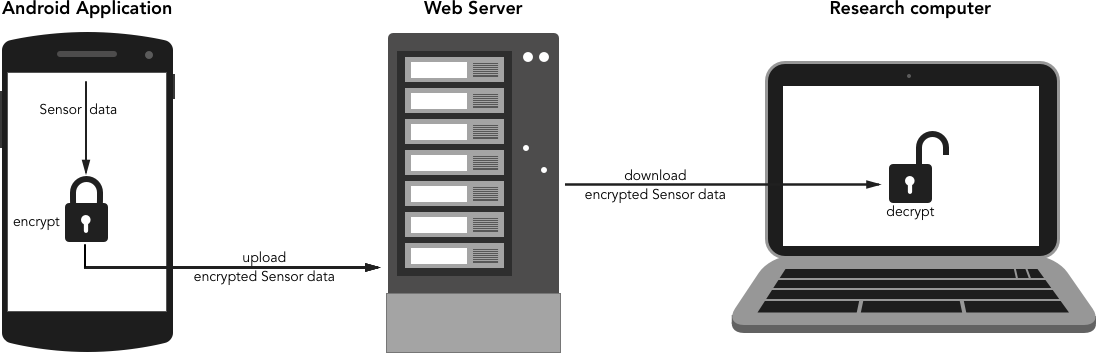
\includegraphics[width=\textwidth]{dataflow}
\caption{Security Dataflow}\label{security}
 	\vspace{10 mm}
\end{figure}

In order to prevent that the participants can be identified by the user id because it is been generated by a SHA256 hash function that is infeasible to invert. In other words, the SHA256 algorithm generates a base16-String from the email-address of the user and there is no mathematical known way to recover the original email address in feasible time from the base16-String. 
\bigbreak
For encrypting the gathered data, the entries are independently getting encrypted before written to the database using a hybrid cryptographic procedure. Hybrid cryptography means the combination of using a the faster and performance friendlier symmetric cryptography (using the same key for encrypting and decrypting) and the slower but more secure asymmetric cryptography. In the asymmetric procedure also known as public-key cryptography, uses two different keys for encrypting and decrypting. A public key is used for the encryption of the data and the private counterpart is used to decrypt the data.
\bigbreak
The encryption is the Android app works as follows:\\
A symmetric key will be generated every time the app starts using the AES CBC algorithm with an PKCS5Padding and a random SHA1 seed. This symmetric key will be used to encrypt the gathered data, while the symmetric key will added to each entry encrypted with the public key of a pre-generated RSA 1024 bit key-pair.\\ 
The private counterpart of the public key will later be used to decrypt the symmetric key. That symmetric key is then used to decrypt the entries. 
The decryption will happen with a separate written Java application locally on a computer.\\
Thus, a decryption within the applications is not possible because the functionality and keys are not even included. 

\section{Server}
The server contains of three different parts, the back-end that handles the REST-full API calls, the MySQL Database and the web-pages for providing information to the participants of the study. 
In this chapter I will just write about the back-end and the web-pages because the Database design is already described in the previous design chapter. 

\subsection{Back-End}
In the PHP script, the data from the POST gets extracted and decoded from JSON to an PHP-Array.\\
If the format of the data is correct, the script connects to the MySQL database and inserts the values into the corresponding table using SQL-Syntax. For each entry a counter is increasing it's value and after completing the insertion, the counter-value gets returned as a response argument. When something wrong happens, the script is responds with an error-code. 

\subsection{Webpages}
The websites are implemented as simple as possible. They are completely static and only for displaying styled text and images. Therefore the implementation is only been done using HTML5 for the structure and CSS3 for styling the fonts, images and visual structuring.\\
Different fonts were embedded using Google-Webfonts from \footnote{\url{https://fonts.google.com}} which are dynamically being loaded at the page load or from the browser cache. 

\section{Tools}
The development of the following tools was necessary to work with the data that can be downloaded from the MYSQL database.

\subsection{Encryption Tool}
The encryption tool is a Java application that is written to decrypt the downloaded encrypted JSON-File of the gathered data.
The simple tool is implemented in Java and is using the IntelliJ interface builder which is based on XML. 
First the tool read the input JSON-File and writes the beginning of the file into the output textfield.\\
Afterwards it is decrypting the symmetric AES-key using the asymmetric RSA-algorithm with the counterpart private-key to the public-key which was used for encrypting. Having the symmetric key allows to decrypt the whole input line by line using the AES decrypting algorithm.
At the end the decrypted entries are written to a new created file and the filepath is been displayed in the text label. 

\subsection{User Separation Tool}
This and the following three tools are written in Python. This tool reads the decrypted text file that has been created by the java decryption tool. First, it creates a SHA256 Hash from a Github username and compares the entries of the text file with it. It only takes the matching entries and writes them to a new text file. 

\subsection{Value Separation  Tool}
This tool can be used to define which of the entries are needed to work with. For example the user can decide just to create an output file with the latitude of the participants location. The selected data and its timestamp gets written in a new text file as well. 

\subsection{Latex Plot Syntax Creating Tool}
This little tool is calculating an average for every Minute of the timestamp of the read text file. As the gathering saved a value every few seconds, it makes no sense to display all the values in a plotted graph.\\
The output contains the timestamp with the value for every minute in a syntax that can directly been interpreted by latex and the pgfplots library. 

\subsection{Map to Duration Tool}
This tool calculates takes a duration and maps the current measurements on that specific duration. That allows to compare the results in a graph independent of the duration the participant needed to solve the task. 

\section{Summary}
In this chapter I describe the implementation of the software and tooling for the experiments. 
\bigbreak
The Android app contains of:
\begin{itemize}
\item Login View - verifies username with Github API
\item Permissions View - asks to grand permissions to app
\item Information View - shows terms of the experiment
\item Gather View - control center for the gathering process (start, stop, send, restart)
\item Question - Asks participants questions and sends to server
\end{itemize}
the next section describes the data gathering in process in detail followed by the implementation of the data storage within the app. The app uses a hybrid encryption using AES and RSA. 
\bigbreak
In the next part I described the simple php implementation with the database connection of the Server backend. For the frontend I used standard HTML and CSS components and Googler web-fonts.
The decryption tool uses RSA and AES for decrypting the data. The other tools read a textfile, manipulate the data and write the results in a new textfile.  
